In this chapter, the scope of this thesis will be defined and a user scenario outlined, split into these sections:

\begin{itemize}
	\item \textbf {Scope Definition and Research Objectives} - Confines the scope of this thesis to a number of research objectives.
	\item \textbf {Selected 2D-Projection Method} - Decides on the algorithms employed for retrieval of artist similarity and generation of 2D layouts, selected from the algorithms described in Chapter ~\ref{ch:relatedwork}.
	\item \textbf {Selected Visualization Method} - Defines which mode of visualization has been selected for the display of visual data to the user, dependent on the previously chosen 2D-projection.
	\item \textbf {Selected Algorithm for Removal of Overlapping of Artists} - Presents the algorithm used for the removal of overlappings in the displayed graph computed by the previously described algorithms.
	\item \textbf {Selected Layout Algorithm for Artist Discovery} - Describes the method which computes the displayed graph's layout when freshly discovered (related) nodes are added to it.
	\item \textbf {Overview of the Assembly of Algorithms and Information Flow} - Provides figures showing the algorithmic components and information flow between them in the prototypical App ("'Andromeda"').
\end{itemize}

\section{Scope Definition and Research Objectives}

The scope of this thesis is defined by the following goals: 

\begin{itemize}
	\item Verification of the selected artist similarity retrieval method being feasible for mobile end user devices.
	\item Verification of the selected artist similarity visualization (2D-projection) method being a sensible choice for mobile end user devices.
	\item Description of the implementation of a prototype (able to perform the selected computation and visualization methods) on the Android mobile OS platform ~\cite{url:android}.
	\item Description of the design and presentation of the results of a user study, in order to test a set of hypotheses evaluating the performance of the implemented prototype ("'Andromeda"') and its visualization approach.
\end{itemize}

\section{Selected 2D-Projection Method}

After consideration of the options for similarity computation in Chapter ~\ref{ch:relatedwork}, the author has concluded that the approach presented in \cite{Morrison:2003:FMS} (combining multi-dimensional scaling by application of a spring model with sampling and interpolation), is a promising approach to the problem of music library visualization, accommodating mobile device processors with low complexity computation. The approach will not be applied unaltered, but modifications and enhancements will be made and described in this thesis, namely in Chapters ~\ref{ch:computation} and ~\ref{ch:implementation}.
It must be noted that this computational method is limited in the amount of objects which can feasibly be displayed (and computed) on a mobile device. Also, since for some data structures no similarity metrics are currently available, the adapted MDS method is not suitable for all kinds of music data. For artist discovery functionality, no related artist ranking is taken into account (for this thesis), so in this case related artists are displayed by implying equal importance (as will be described in section ~\ref{sec:selected-algorithm-discovery}.

\section{Selected Visualization Method}

Since an MDS computation approach has been selected for further proceeding, the visualization computation for a music collection is entangled with the similarity computation and cannot be freely chosen. Also, the presentation space for visualization is chosen to be two-dimensional, because three-dimensional visualizations are hard to quickly browse by the user due to mobile devices' small screen estate. Thus, the visualization method for object clusters is constrained to be a two-dimensional layout algorithm, positioning the laid-out objects such that they resemble the coordinates generated by MDS (by application of a spring model). For ease of navigation, zooming and panning will be added, and images will be used for faster identification of object types.

\section{Selected Algorithm for Removal of Overlapping of Artists}

The computational methods described previously generate a 2D model of the user's music library, but they disregard the fact that the presented objects may overlap. In order to separate objects from each other visually, an algorithm needs to be implemented that produces an overlap free model. Obviously, the definition of overlapping depends on the size of the objects as they are presented in the viewport.

The author of this thesis decided to use an iterative approach to the removal of overlappings - a modification and simplification of the idea of the force-transfer algorithm \cite{Huang03force-transfer:a}. Graph nodes are added into a fresh space, one by one, and while they are added, they are positioned such that overlappings with other nodes are eliminated. This elimination is performed by moving the freshly added node on the vector [overlapped node's center TO added node's center] so far that they don't overlap anymore. As this might create new overlappings, several iterations of this "'pushing away"' are performed, until the freshly added node does not overlap any other nodes. The outcome of this algorithm is a cleanly laid out representation of the previously crowded MDS computation outcome. This approach has shortcomings which are described in section ~\ref{subsec:libraryvis}.

\section{Selected Layout Algorithm for Artist Discovery}
\label{sec:selected-algorithm-discovery}

A graph of artists during artist discovery is star-shaped initially: In the center is the seed artist, for whom the user wants related artists shown. Around the seed artist, the seed's related artists are arrayed with equal distances to the seed - they are "'owned"' by the seed. But, if the user chooses to display related artists of an artist that is currently shown as a related artist, then this one becomes another seed artist. This new seed artist will receive its own related artists, while still being connected to the original (first) seed. It would not do to calculate such a graph deterministically - such an algorithm would be too rigid in case distances between artists need to be changed, or even have to change dynamically. So, a force-directed layout algorithm is chosen, where all artists push away from each other, but the related artists which are no seeds are attracted by their owning seeds (as described in \cite{Kobourov04}). These forces are applied continuously in iterations, as long as a certain movement threshold has not been undercut. After the optimal parameters for these forces have been found, such an algorithm can handle an arbitrary number of displayed artists and seed artists.

\section{Overview of the Assembly of Algorithms and Information Flow}

To give the reader a better picture of the sections to come, an overview is given in Fig. ~\ref{fig:algorithm_flow_visualization} which explains how the selected algorithms process and pass on information to each other. The process is as follows:

\indent After the extraction of music metadata stored on the device, it is matched with the metadata of music titles which can be found for the corresponding music entities (artists, albums, titles) in web sources (Last.fm, Echonest). This is based on a simple web API search, selecting the first match that is returned by the API, letting the web API take care of spelling errors (duplicates are not removed). Subsequently, artist similarity measures are extracted from web sources, concretely only from Last.fm, since Echonest currently does not offer these values. Artist similarity data is then completed via interpolation. The artists for whom metadata could be found in web sources are then laid out in 2D space with a multi-dimensional scaling algorithm by application of a spring model: A distance matrix of all artists is built up using the retrieved similarity measures, then seed artists are laid out according to spring model forces, then remaining artists are positioned around the seeds, and finally the spring model algorithm is applied on all artists for a few iterations. After the spring model algorithm has finished, overlappings of artists are removed, and all artists are rendered on the device's screen with OpenGL. The visualization then continuously reacts to the user's actions until the process is terminated.
An in-depth explanation of these information flows is given in Chapter ~\ref{ch:implementation}.

\subsection{Library Visualization}

\begin{figure}[H]
  \centering
    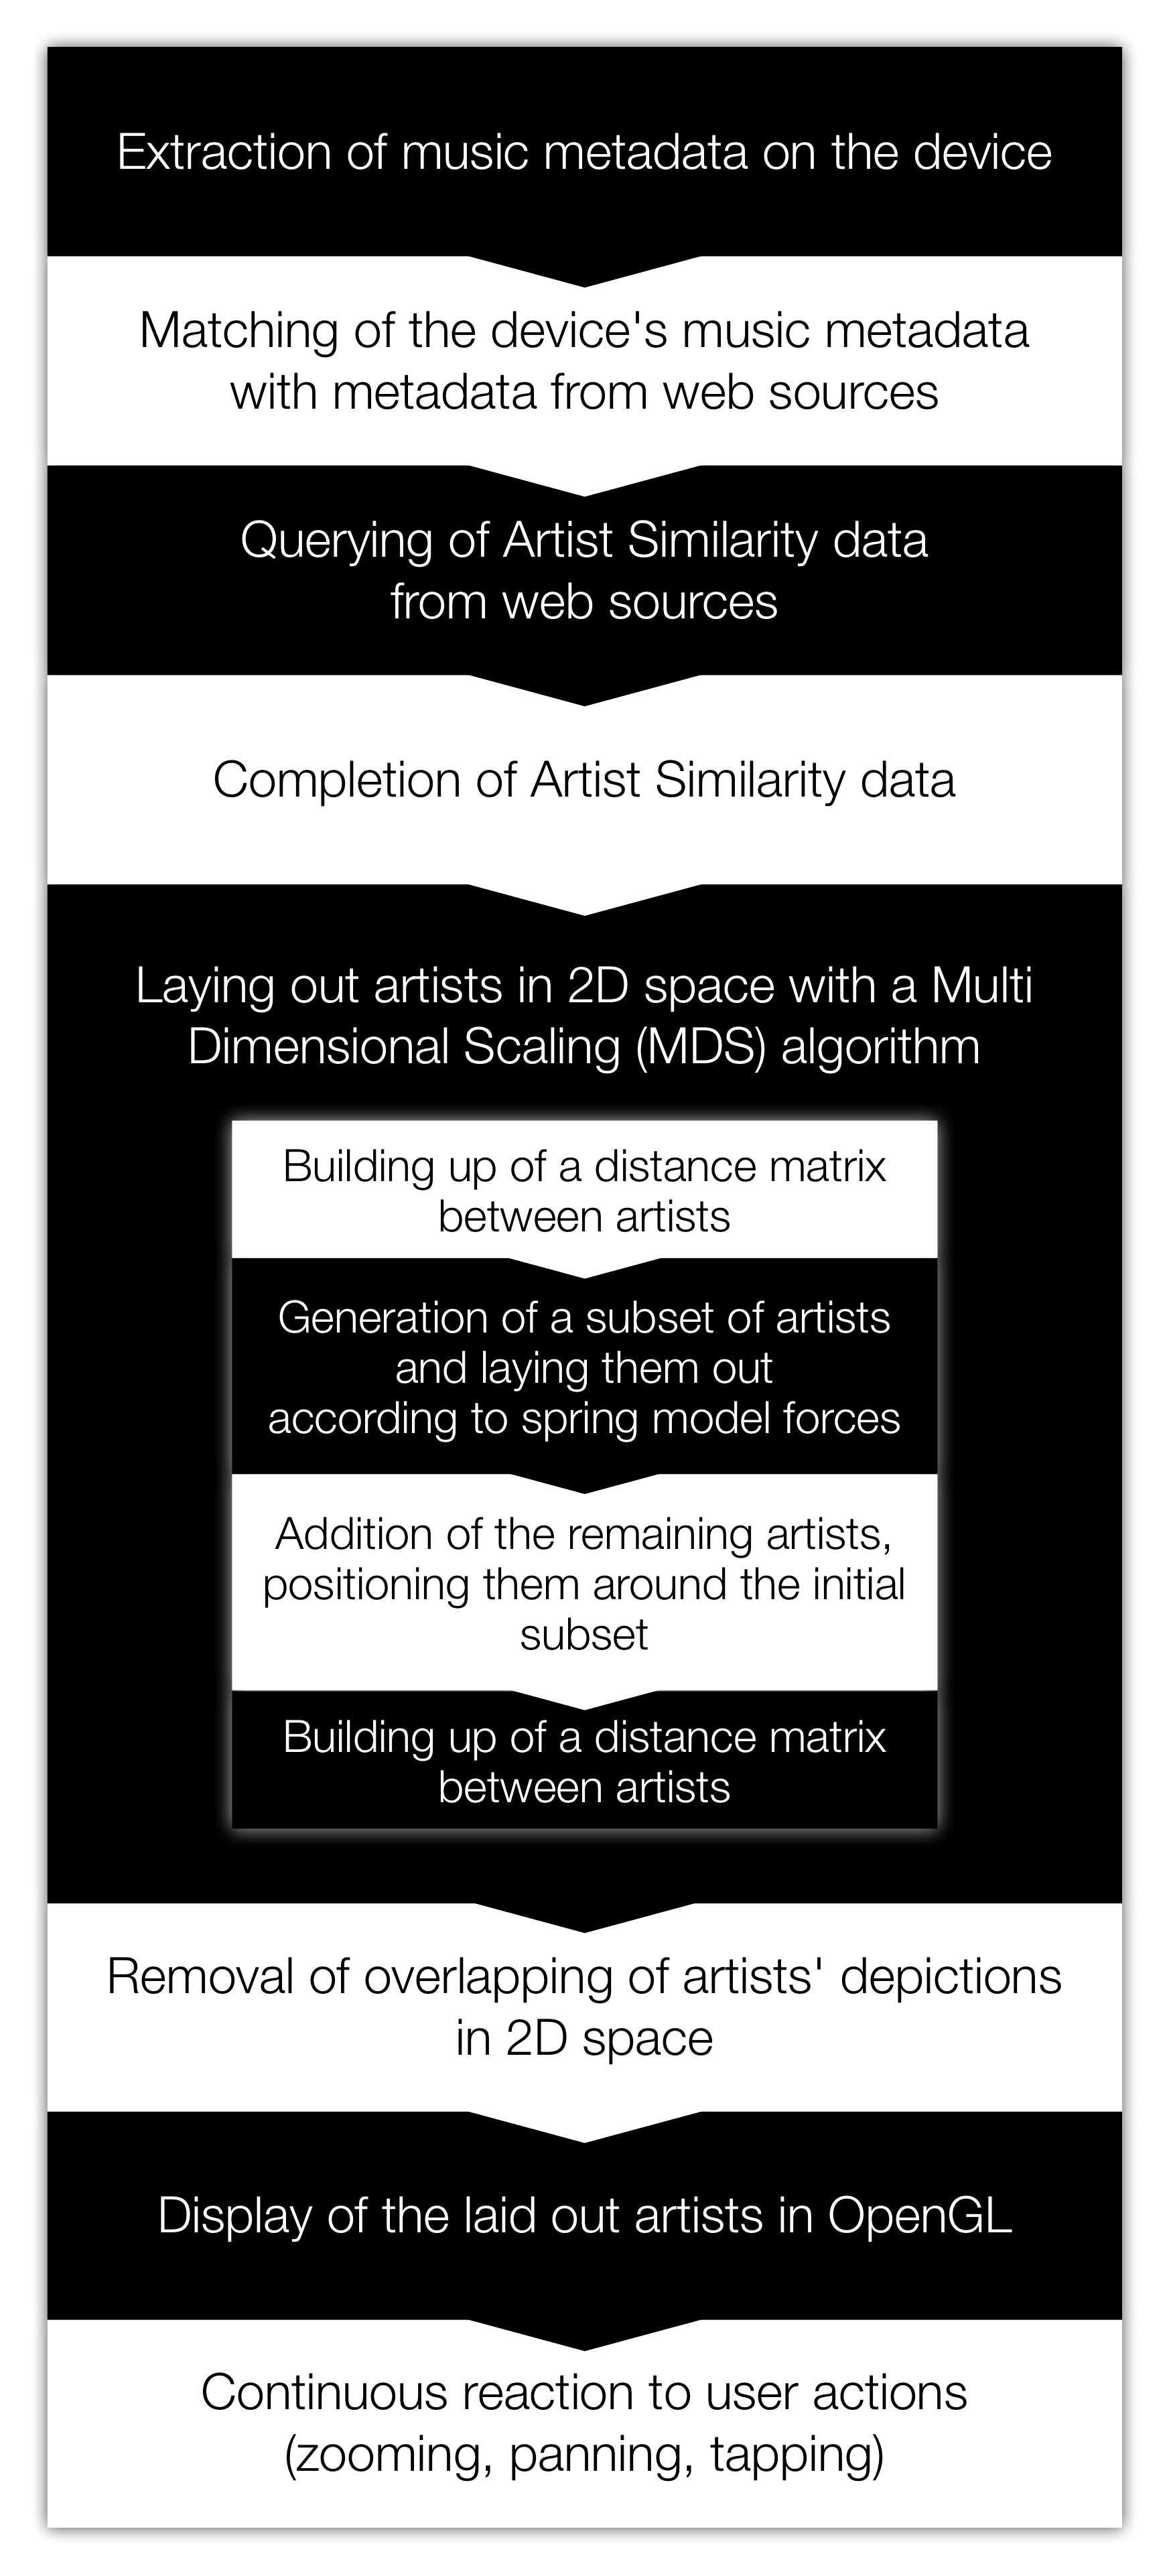
\includegraphics[width=0.45\textwidth]{figures/algorithm_flow_visualization}
  \caption{Algorithms for Library Visualization}
  \label{fig:algorithm_flow_visualization}
\end{figure}

\subsection{Artist Discovery}

Artist discovery is initiated by the user selecting a certain artist ("'subject"'), and requesting discovery mode. At first, a similarity ranking list is retrieved from Last.fm, then the top 5 similar artists are added to the graph layout (at randomized positions), and then all artists (initially, only the seed node and the 5 most similar artists; later on, more seed nodes and related artists can be added) are continuously laid out by a force-directed layout algorithm.

\begin{figure}[H]
  \centering
    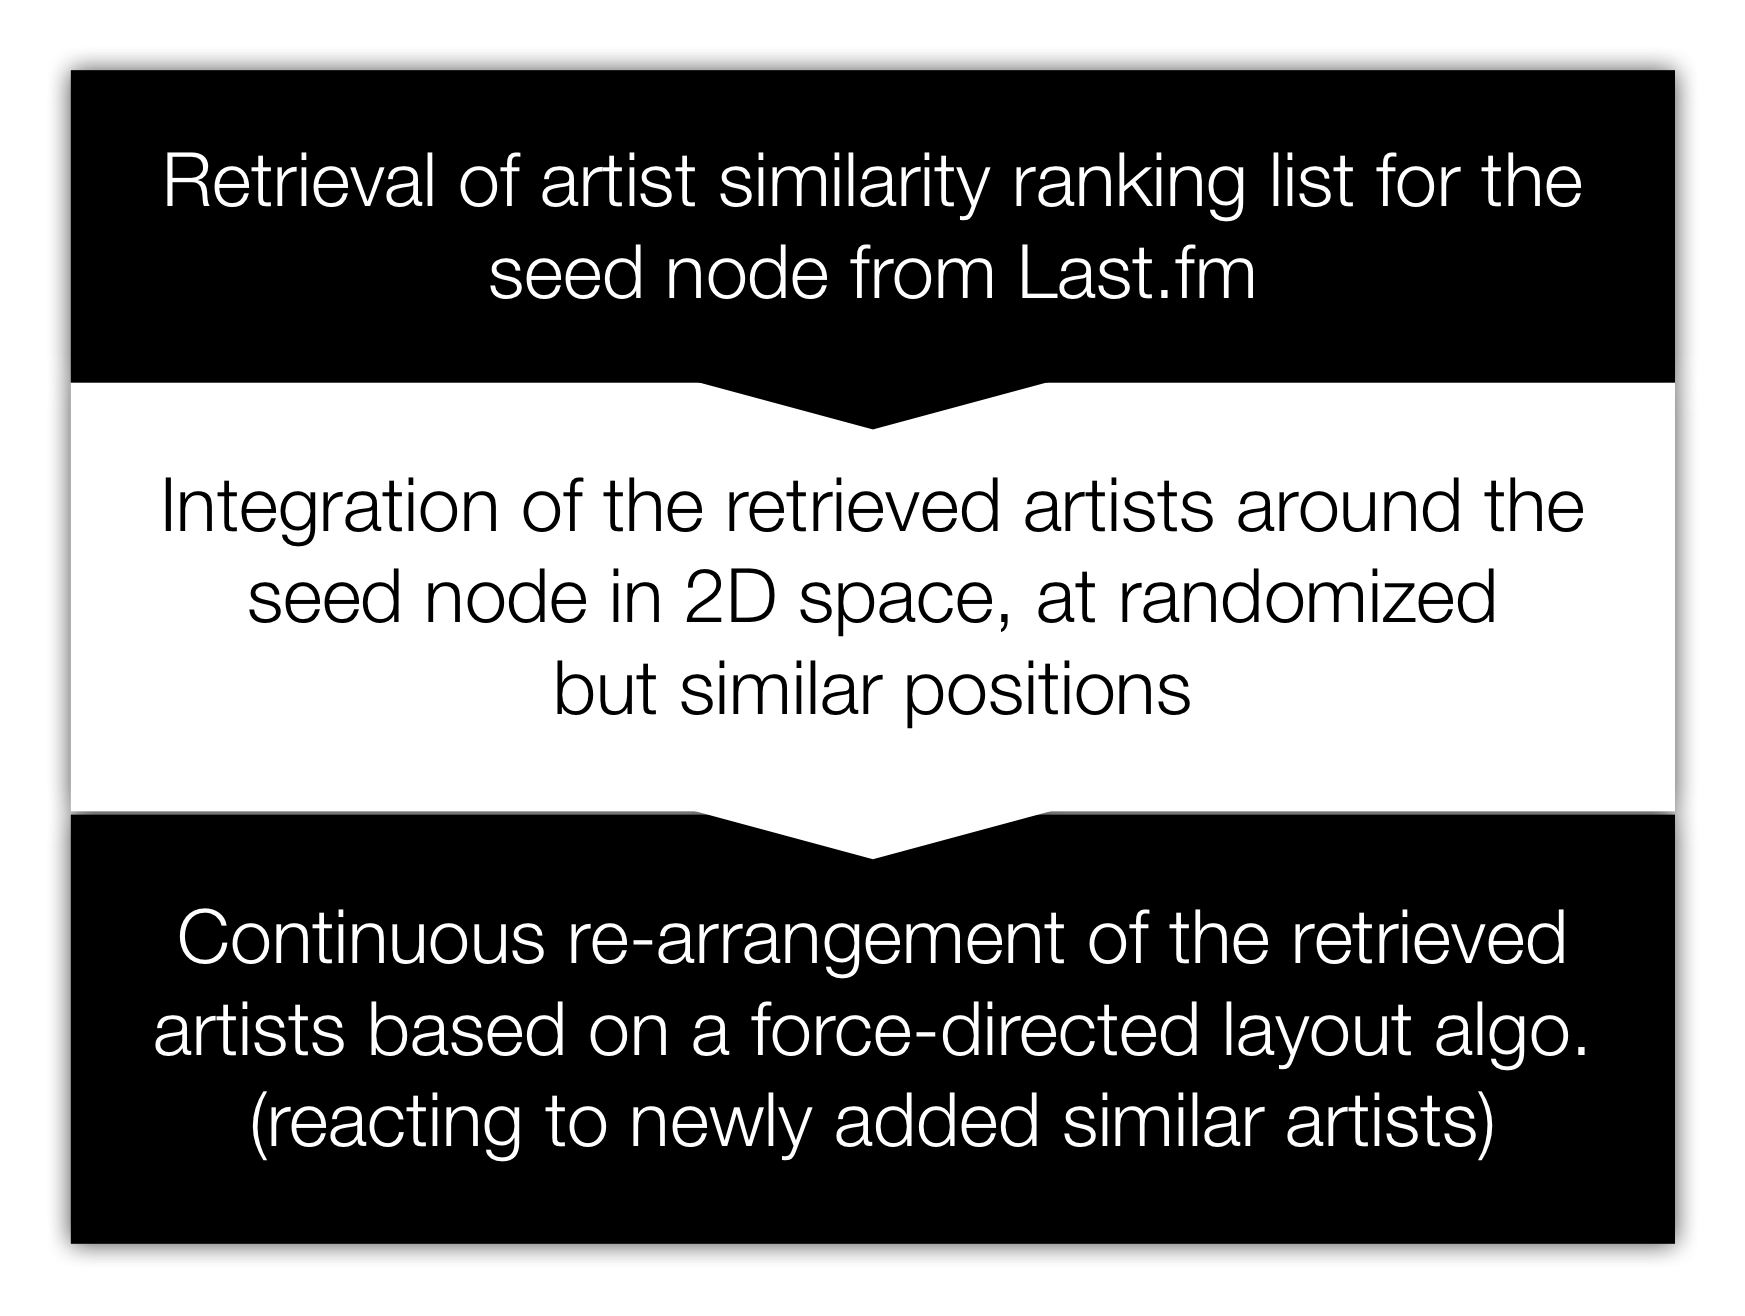
\includegraphics[width=0.45\textwidth]{figures/algorithm_flow_artist_discovery}
  \caption{Algorithms for Artist Discovery}
  \label{fig:algorithm_flow_artist_discovery}
\end{figure}

\section{Summary}

After the definition of the scope of this thesis (verification of artist similarity retrieval methods and their implementation in a prototype called "'Andromeda"'), algorithms have been selected for further usage which have already been outlined in Chapter ~\ref{ch:relatedwork}. For the computation of 2D layouts based on artist similarity, a multi-dimensional scaling method (by application of a spring model) has been chosen, and the accompanying visualization is highly dependent on the computational part - therefore, a straightforward 2D layout of the MDS (spring model) output has been selected as visualization. 
While the algorithm for the removal of node overlappings in the graph resulting from the previously mentioned computation is a modification of a force-transfer algorithm, the layout computation for artist discovery has been chosen to be force-directed. Finally, an overview of the algorithms and information flow between them has been given, for both artist similarity visualization and artist discovery.